%%%%%%%%%%%%%%%%%%%%%%%%%%%%%%%%%%%%%%%%%%%%%%%%%%%%%%%%%%%%%%%%%%%%%%
\chapter{Metodologia}
%%%%%%%%%%%%%%%%%%%%%%%%%%%%%%%%%%%%%%%%%%%%%%%%%%%%%%%%%%%%%%%%%%%%%%
A metodologia do presente trabalho é dividida em 3 principais partes. A primeira é a etapa apresenta um fluxograma de operação do sistema que ajuda a nortear a especificação das demais etapas. É na segunda etapa que ocorre a definição dos componentes de hardware que compões o dispositivo. Já na terceira etapa, são abordados as características e principais fatores que devem ser empregados no desenvolvimento do software do dispositivo.



%%%%%%%%%%%%%%%%%%%%%%%%%%%%%%%%%%%%%%%%%%%%%%%%%%%%%%%%%%%%%%%%%%%%%%
\section{Fluxograma de operação}
%%%%%%%%%%%%%%%%%%%%%%%%%%%%%%%%%%%%%%%%%%%%%%%%%%%%%%%%%%%%%%%%%%%%%%
De modo a entender as condições de operação do sistema como um todo, elaborou-se um fluxograma das suas interações. Sendo possível desta forma perceber os pontos críticos para comunicação e interfaceamento da cadeia logística em cada etapa do processo.
\begin{figure}
  \caption{Fluxograma de operação do sistema}
  \begin{center}
      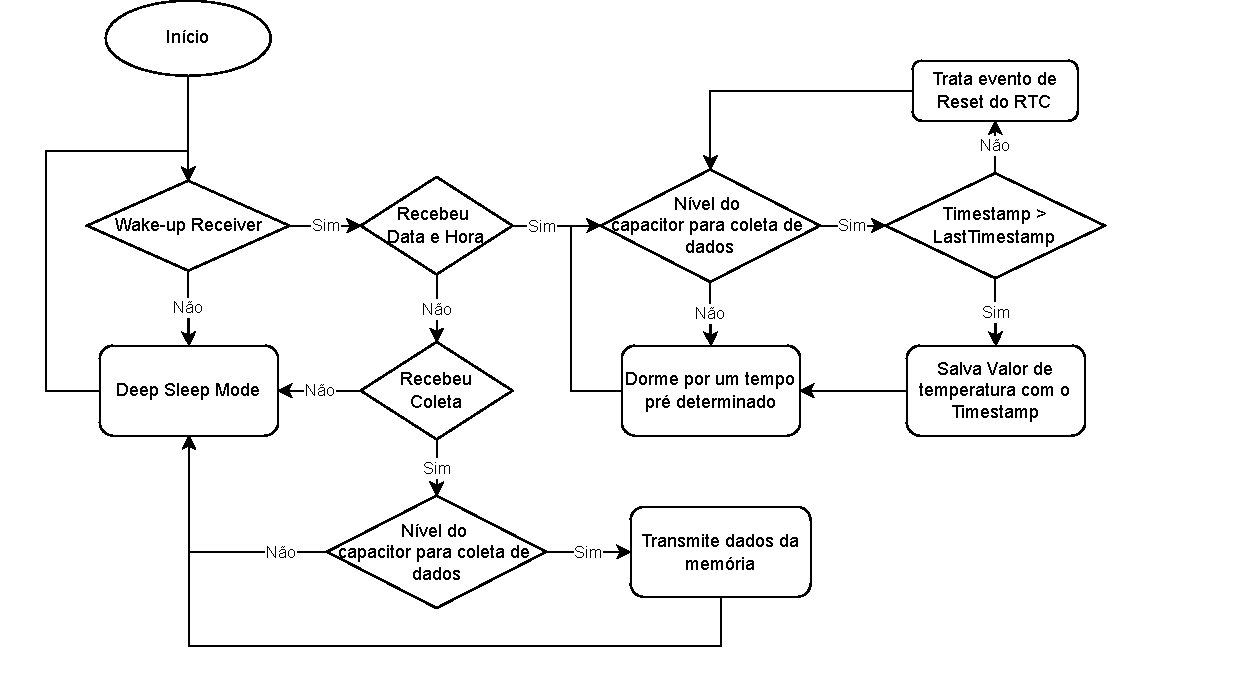
\includegraphics[scale=0.7]{img/fluxogramaOperacao.drawio.pdf}
  \end{center}
  \fonte{Elaborado pelo autor}
  \label{fig:fluxo}
\end{figure}

Um exemplo claro e notório deste tipo de avaliação se dá na inclusão de um bloco de verificação da tensão acumulada no capacitor de retensão. Com isso, se espera manter um nível mínimo de potência para manter o calendário vivo.
Na figura~\ref{fig:fluxo} pode-se ver a representação completa deste fluxo de operação.Além disso, se faz preciso a inclusão de um bloco para configuração inicial do sistema, já que informações anteriores precisam ser descartadas e isso pode ser feito simplesmente com o início de uma inserção da hora do sistema.


%%%%%%%%%%%%%%%%%%%%%%%%%%%%%%%%%%%%%%%%%%%%%%%%%%%%%%%%%%%%%%%%%%%%%%
\section{Hardware}
%%%%%%%%%%%%%%%%%%%%%%%%%%%%%%%%%%%%%%%%%%%%%%%%%%%%%%%%%%%%%%%%%%%%%%
Após a modelagem apresentada no referencial teórico, torna-se possível especificar os requisitos do dispositivo eletrônico capaz de executar as operações citadas no fluxograma de operação da figura~\ref{fig:fluxo}. Neste capítulo será detalhado cada parte do hardware proposto mostrado na figura~\ref{fig:sistema}.

\begin{figure}
  \caption{Diagrama de blocos dos componentes do hardware.}
  \begin{center}
      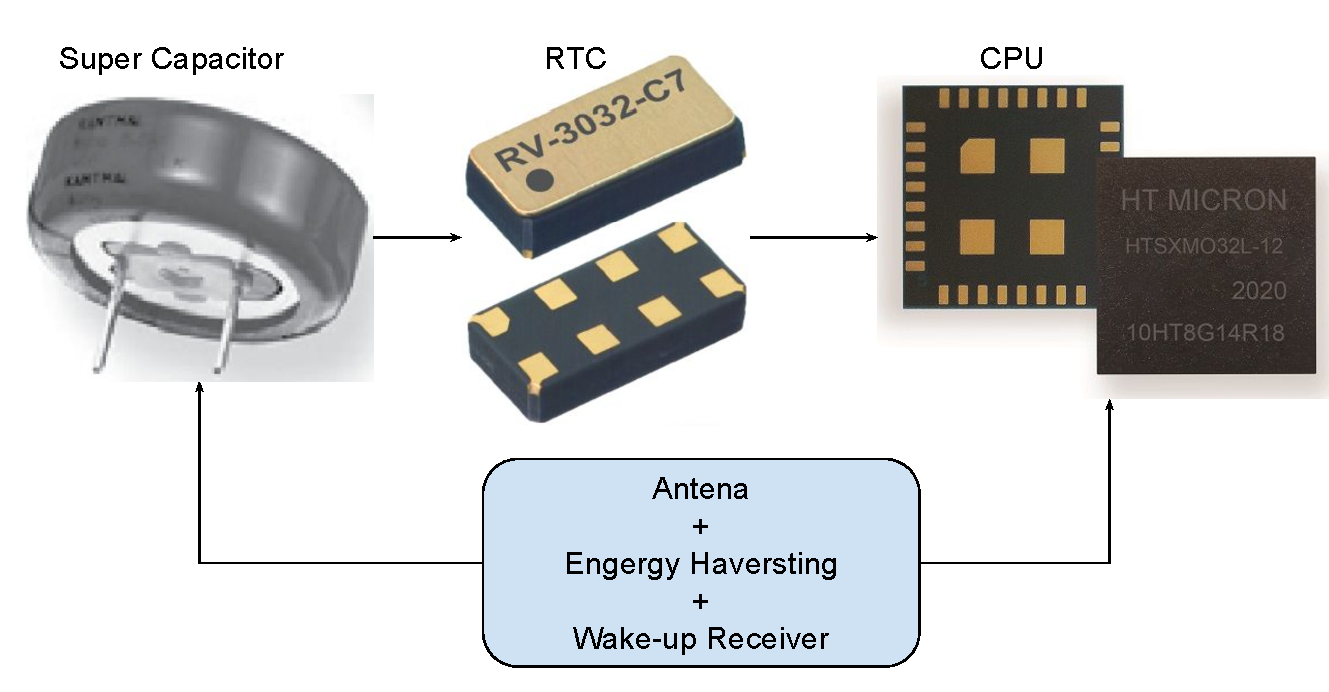
\includegraphics[scale=0.7]{img/sistema.pdf}
  \end{center}
  \fonte{Elaborado pelo autor}
  \label{fig:sistema}
\end{figure}
%%%%%%%%%%%%%%%%%%%%%%%%%%%%%%%%%%%%%%%%%%%%%%%%%%%%%%%%%%%%%%%%%%%%%%
\subsection{RTC}
%%%%%%%%%%%%%%%%%%%%%%%%%%%%%%%%%%%%%%%%%%%%%%%%%%%%%%%%%%%%%%%%%%%%%%
Aplicações de monitoramento de temperaturas em dispositivos IoT muitas vezes~\cite{Soh} podem contar com a definição de hora e data baseados no momento da transmissão, sendo dispensável a estes o uso de circuitos com \textit{Real Time Clock}(RTC), relógios de tempo real. Nos casos em que a janela de transmissão de dados ocorre um momentos distintos da coleta dos mesmos, um marcação de tempo se faz necessária para garantir a procedência desta coleta.

Para garantir essa marcação de tempo neste projeto, procurou-se obter um circuito de RTC capaz de manter sua funcionalidade por logos períodos de temo com um consumo mínimo de potência. Dentre as solução pesquisadas, cabe um destaque especial para o RV-3032~\cite{rtc} da empresa \textit{Micro Crystal} que combina um circuito integrado (CI) do tipo CMOS com um cristal ressonador interno. 

Este RTC funciona sob vácuo em embalagem cerâmica hermeticamente fechada com tampa metálica. Seu consumo de corrente em operação chega a níveis consideravelmente baixos, da ordem de nano amperes (nA). Além disso, o mesmo possuis uma compensação da precisão em função da temperatura (TXCO), que garante uma precisão de $\pm 2.5ppm$ em toda a faixa de $-40^oC$ até $85^oC$.

\begin{figure}
  \caption{Curva de operação do RV-3032}
  \begin{center}
      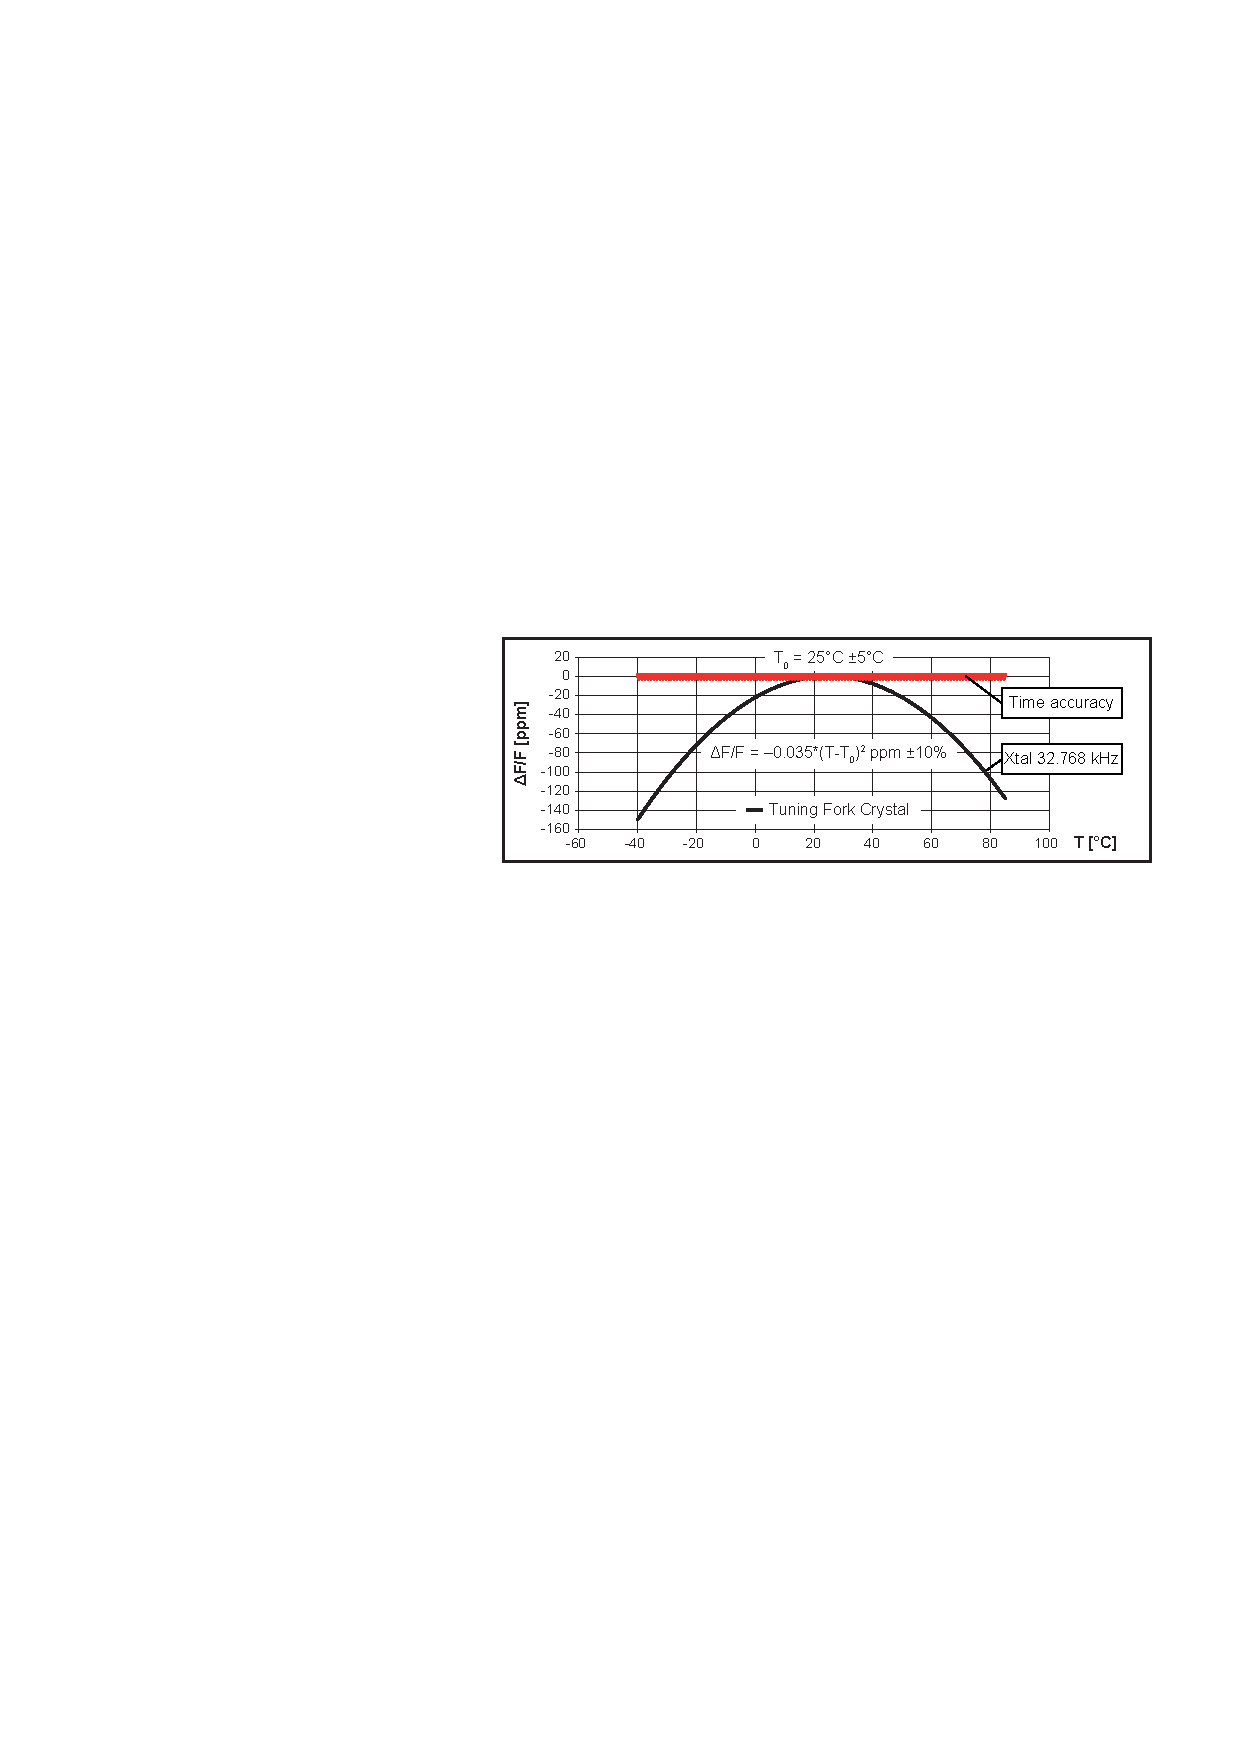
\includegraphics[scale=0.8]{img/RTCcurva.pdf}
  \end{center}
  \fonte{\citeonline{rtc}}
  \label{fig:RTC}
\end{figure}
A inserção de um sensor de temperatura e do cristal dentro do RV-3032 além de aumentar a precisão fora da temperatura convencional de $25~C$, possibilita o uso desta informação de temperatura para dispositivos IoT que possam fazer esse tipo de aquisição.
Este sensor possui uma acurácia típica de $\pm 1^oC$ que é relativamente alta, mas que não apresenta prejuízos para o estudo proposto, uma vez que a temperatura aproximada se faz suficiente para este tipo de controle.
Outra vantagem do uso deste RTC nesta aplicação, se dá em função da possibilidade de configuração de alarmes capazes de acordar o processador por uma janela de tempo pré estipulada, ou o cruzamento por uma temperatura específica. Esta função, pode ser considerada um real diferencial para a redução do consumo de operação do dispositivo, já que permite ao microcontrolador ligado ao RTC entrar em um modo profundo de economia de energia (\textit{Deep Sleep Mode}).

%%%%%%%%%%%%%%%%%%%%%%%%%%%%%%%%%%%%%%%%%%%%%%%%%%%%%%%%%%%%%%%%%%%%%%
\subsection{Super capacitor}
%%%%%%%%%%%%%%%%%%%%%%%%%%%%%%%%%%%%%%%%%%%%%%%%%%%%%%%%%%%%%%%%%%%%%%
Dispositivos IoT podem operar de duas maneiras, conectados em algum sistema de alimentação por fios, ou alimentados para uma fonte de energia conectada somente a ele. Devido às características de mobilidade do sistema proposto neste projeto, a alimentação por algo conectado a rede elétrica não se faz possível, sendo assim necessário o uso de alguma fonte de alimentação independente.

Embora o sistema de coleta de energia dos sinais de RF estejam sempre operando, a potência capturada por este não se faz capaz de operar as funções básicas do RTC ou do microcontrolador.
Resta neste caso, recorrer a um dispositivo que armazene esta energia. Tradicionalmente, dispositivos IoT deste tipo possuem uma bateria para solucionar esta questão. Porém, baterias tendem a sofrer depreciação ao se executar cargas e descargas com uma frequência muito alta. 

Em um estudo realizado por \citeonline{supercap}, concluiu-se que o uso de super capacitores em sistemas de coleta de energia por RF pode ser uma alternativa razoável, pois embora eles possuam uma densidade de acumulo de carga centenas de vezes menores que baterias, eles se mostram eficientes em situações de carga e descarga. Neste mesmo artigo, mediu-se o tempo de carga de um capacitor e três Faraday sendo notado um tempo de cargar de aproximadamente três horas para um dispositivo comercial de conversão de energia.

Para avaliar a curva de carga e descarga do capacitor, tem-se que considerar os princípios básicos deste componente, como a relação $RC$ também chamada de constante tau ($\tau$). Na tabela~\ref{tb:capacitor} estes valores são apresentados e a partir deles, pode-se obter a curva apresentada na figura~\ref{fig:capacitor}.

% Please add the following required packages to your document preamble:
% \usepackage{booktabs}
\begin{table}
\begin{center}
\caption{Valores de $\tau$.}
\begin{tabular}{@{}cccc@{}}
\toprule
 & \textbf{$t$}  &\textbf{ $v(t)/V_0$} & \\ \midrule
 & $1\tau$ & $0,36788$ & \\
 & $2\tau$ & $0,13534$ & \\
 & $3\tau$ & $0,04979$ & \\
 & $4\tau$ & $0,01832$ & \\
 & $5\tau$ & $0,00674$ & \\ \bottomrule
\end{tabular}
\end{center}  
\fonte{Adaptado de \citeonline[p.~246]{Alexander2013}}
\label{tb:capacitor}
\end{table}

\begin{figure}
  \caption{Curva de carga característica de um capacitor.}
  \begin{center}
      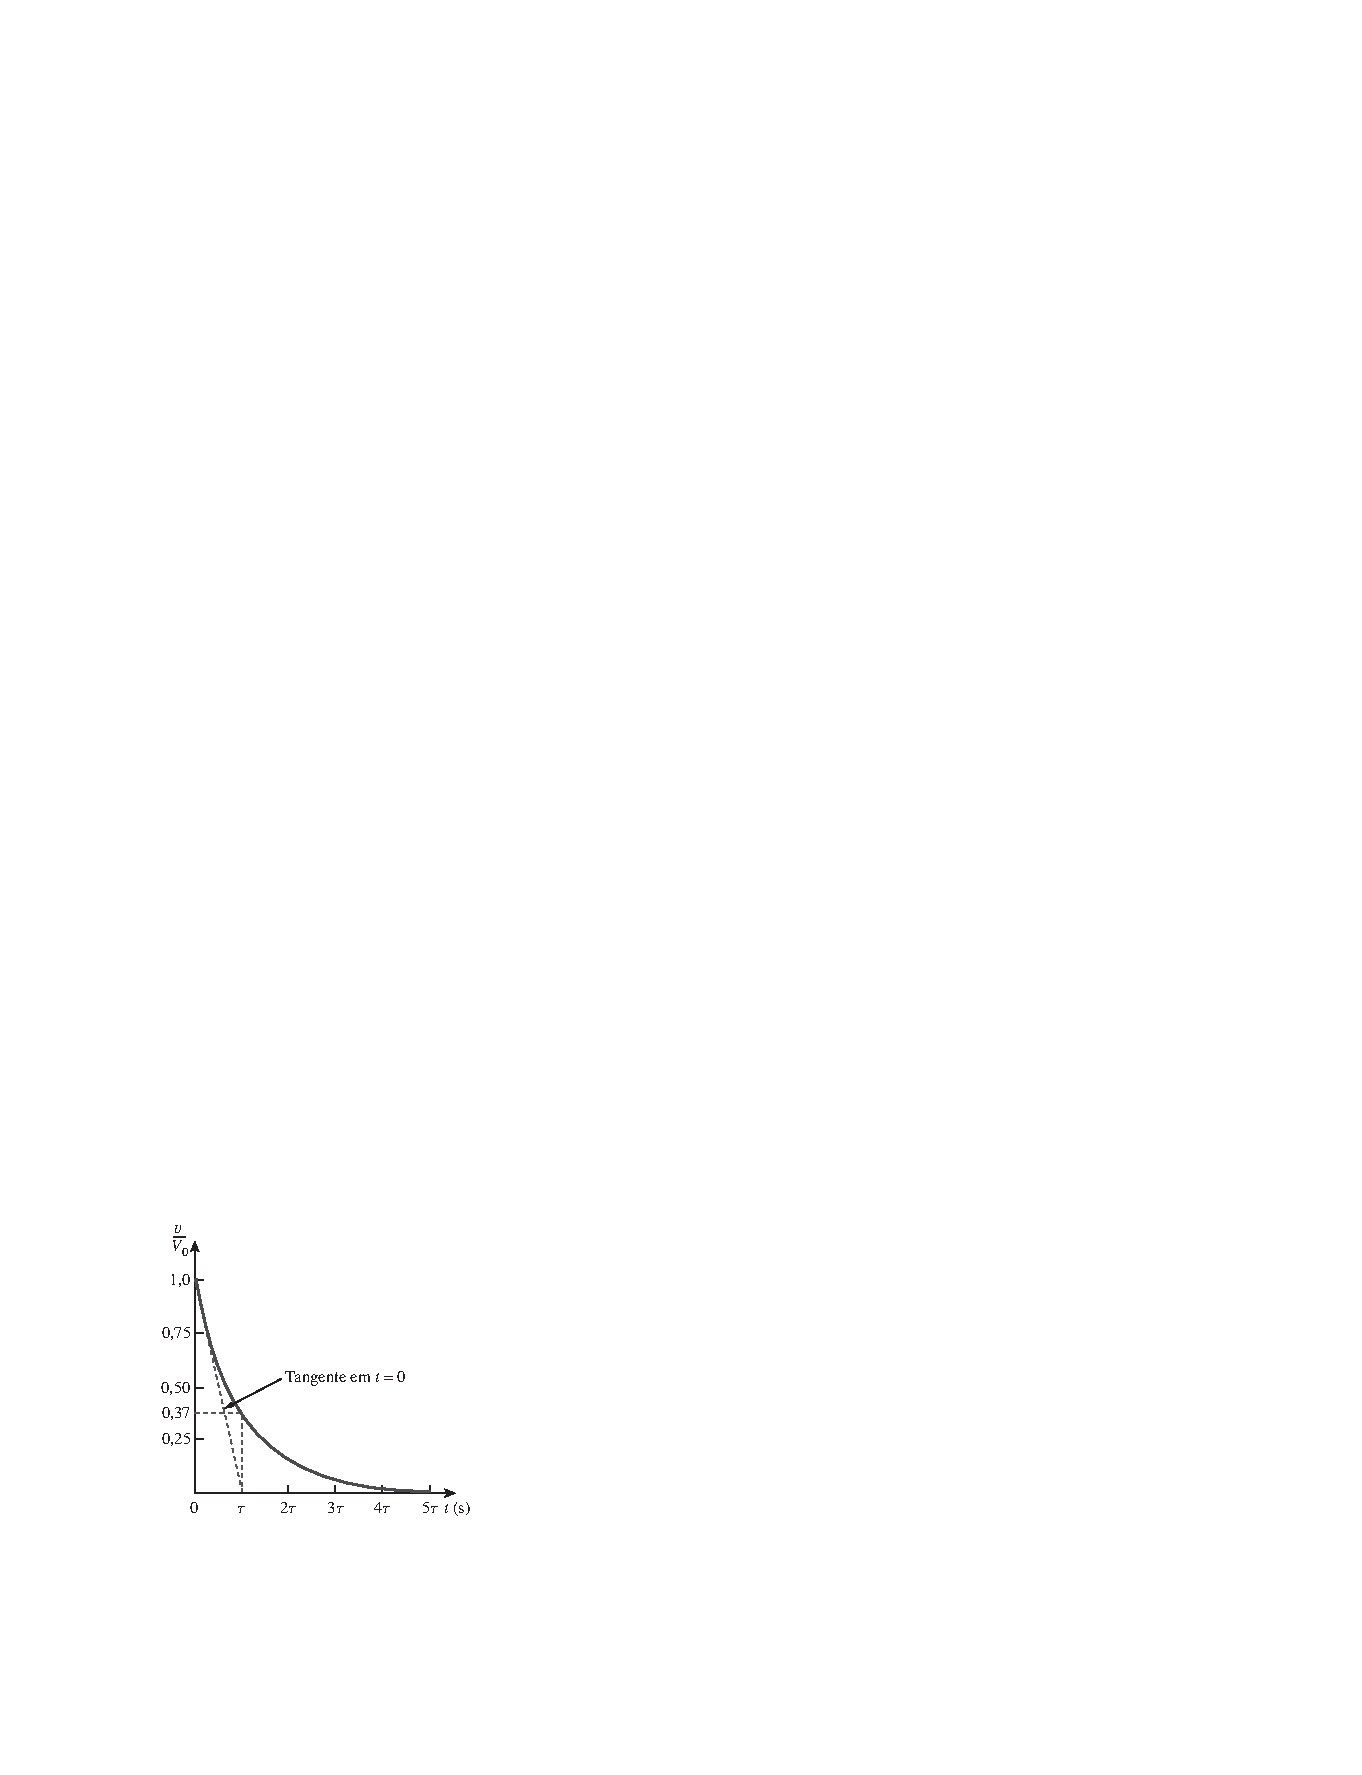
\includegraphics[scale=1]{img/capacitor.pdf}
  \end{center}
  \fonte{\citeonline[p.~246]{Alexander2013}}
  \label{fig:capacitor}
\end{figure}

Já para estimar o valor ideal de capacitor a ser empregado nesta solução, considerou-se a corrente máxima de $240nA$ do RTC de acordo com a informações do datasheet citado no tópico RTC. A partir disso, e considerando o range de tensão de operação ente $1,3V$ a $5$.

Com isso, obteve-se inicialmente o delta de tensão de operação através da equação\ref{eq:dv}.



\begin{equation}
    \Delta V = V_{cc}-V_{min}
  \label{eq:dv}
\end{equation}


Onde $V_{cc}$ é a tensão de entrada e $V_{min}$ é a tensão mínima de operação do RTC.

\begin{equation}
     \Delta V =5V-1,3V = 3,7V
\end{equation}

A partir da equação do tempo de descarga, pode-se obter o valor do capacitor considerando um tempo de retensão de aproximadamente 40 dias. Estipulou-se um tempo demasiado alto para garantir longos períodos de tempo sem o recebimento de energia através do coletor. A equação~\ref{eq:T} define o cálculo do tempo e transformando na equação~\ref{eq:C} calcula-se o capacitor


\begin{equation}
    T=\frac{\Delta V \times C}{I}
  \label{eq:T}
\end{equation}

Onde $T$ é o tempo em segundos, $\Delta V$ é a variação da tensão de operação do RTC, $I$ é a corrente de operação do RTC e $C$ é o capcitor a ser calculado.

\begin{equation}
    C=\frac{(40 Dias\times 60\times60\times24) \times 240nA}{3,7V} = 224mF \cong 220mF
      \label{eq:C}
\end{equation}

O capacitor foi aproximado para um valor comercial e após uma busca em distribuidores de componentes, escolheu-se pelo \textit{Part Number} LM055224A~\cite{Ohmite}.


%%%%%%%%%%%%%%%%%%%%%%%%%%%%%%%%%%%%%%%%%%%%%%%%%%%%%%%%%%%%%%%%%%%%%%
\subsection{HT32SX}\label{sc:HT32SX}
%%%%%%%%%%%%%%%%%%%%%%%%%%%%%%%%%%%%%%%%%%%%%%%%%%%%%%%%%%%%%%%%%%%%%%
O iMCP–HT32SX é um circuito integrado multicomponente (MCO) projetado para fornecer uma solução de conectividade pronta para uso para aplicativos de Internet das Coisas (IoT). Ele fornece comunicações de uplink (transmissão) e downlink (recepção), e é o primeiro produto HT Micron em uma nova família de componentes sem memória. Suas pequenas dimensões, alto desempenho e baixo consumo de energia visam a melhor experiência para desenvolvedores de IoT. Possui um ARM Cortex M0+ de 32 bits (STM32L052x8) e o transceptor de baixa potência S2-LP da ST Microelectronics combinado com o SKY66420 da Skyworks Solutions que oferece todas as vantagens de desempenho, integração e conveniência da tecnologia avançada de empacotamento de semicondutores em um único chip. Este chip possui também uma EEPROM com capacidade para armazenar 2k Bytes. Na figura~\ref{fig:blockHT32SX} pode-se ver o diagrama de blocos do iMCP-HT32SX desenvolvido pela empresa HT Micron.

\begin{figure}
  \caption{Diagrama de blocos do iMCP–HT32SX.}
  \begin{center}
      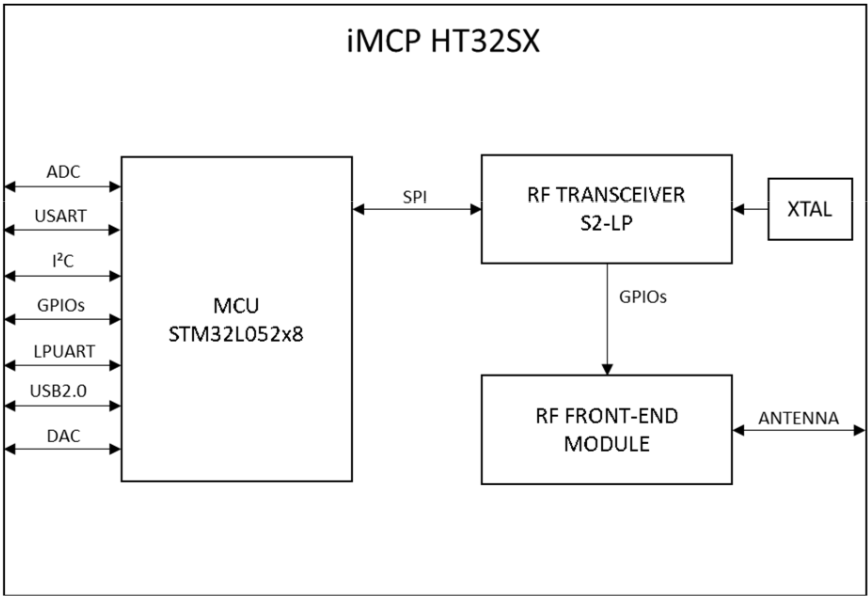
\includegraphics[scale=0.5]{img/imcpHT32sx.png}
  \end{center}
  \fonte{HT Micron\cite{Ht32sx2021} }
  \label{fig:blockHT32SX}
\end{figure}

Além dos requisitos já citados, o HT32SX ainda conta com um sensor de temperatura interno, que poderia ser utilizado para o log de eventos e assim poder-se traçar a curva desta. Porém, devido a disponibilidade de um sensor de temperatura dentro do RTC, optou-se por utilizar este e assim evitar a retirada do modo profundo de economia de energia do microcontrolador para executar esta tarefa.
%%%%%%%%%%%%%%%%%%%%%%%%%%%%%%%%%%%%%%%%%%%%%%%%%%%%%%%%%%%%%%%%%%%%%%
\subsection{HTSXMO32L-22}
%%%%%%%%%%%%%%%%%%%%%%%%%%%%%%%%%%%%%%%%%%%%%%%%%%%%%%%%%%%%%%%%%%%%%%
A Placa de Avaliação iMCP HTSXMO32L-22 foi projetada para ser uma plataforma de desenvolvimento e facilitar o primeiro contato de novos usuários com o iMCP HT32SX, além de fornecer ao usuário avançado para começar a programar e desenvolver produtos imediatamente com estrutura mínima. Todos os recursos do HT32SX estão disponíveis na placa de avaliação. Duas opções de alimentação podem ser usadas: conexão USB ou bateria externa. A placa de avaliação muda automaticamente para alimentação USB quando esta estiver disponível, possibilitando praticidade na validação do software em fase de testes.  Na figura~\ref{fig:placaHT32SX} pode-se ver a Placa iMCP HTSXMO32L-22 desenvolvida pela empresa HT Micron.

\begin{figure}
  \caption{Placa iMCP HTSXMO32L-22.}
  \begin{center}
      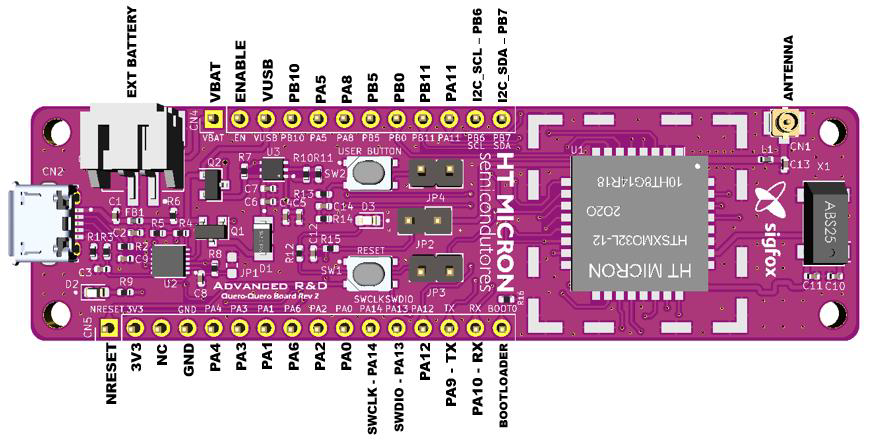
\includegraphics[scale=0.5]{img/placa.png}
  \end{center}
  \fonte{HT Micron\cite{HTSXMO32L} }
  \label{fig:placaHT32SX}
\end{figure}

A conexão para bateria externa torna a placa de avaliação portátil, facilitando testar a conectividade do Sigfox em qualquer lugar que se vá. Como mencionado na secção~\ref{sc:HT32SX}, a substituição de baterias por um super capacitor se fara presente nesta conexão. Os barramentos laterais possibilitam acesso direto as pinos de entradas e saídas. Com isso, a integração entre as diferentes partes do protótipo inicial pode ser efetuada sem necessidade de modificações complexas.

Como se espera uma utilização mínima de espaço nesta aplicação, o uso de antena externa será feito inicialmente. Uma vem que a solução apresente resultado favorável, esta pode ser alterada para uma antena de circuito impresso juntamente com a integração de todos os recursos de hardware. 
%%%%%%%%%%%%%%%%%%%%%%%%%%%%%%%%%%%%%%%%%%%%%%%%%%%%%%%%%%%%%%%%%%%%%%
\subsection{Desempenho energético}
%%%%%%%%%%%%%%%%%%%%%%%%%%%%%%%%%%%%%%%%%%%%%%%%%%%%%%%%%%%%%%%%%%%%%%


%%%%%%%%%%%%%%%%%%%%%%%%%%%%%%%%%%%%%%%%%%%%%%%%%%%%%%%%%%%%%%%%%%%%%%
\section{\textit{Software}}
%%%%%%%%%%%%%%%%%%%%%%%%%%%%%%%%%%%%%%%%%%%%%%%%%%%%%%%%%%%%%%%%%%%%%%
Após a modelagem, deve-se implementar o modelo de software baseado nos levantamentos do fluxograma de operação mostrado na figura~\ref{fig:fluxo}. A partir da documentação e bibliotecas de exemplo contido no repositório do fabricante do módulo HTSXMO32L-22, tornou-se possível escolher entre os modelos uma solução adequada para este projeto.
Dentre as soluções oferecidas, selecionou-se a \textit{P2P Demo Application} devido a sua simplicidade de operação e possibilidade de adaptação para as necessidades do projeto. Na figura~\ref{fig:p2p} pode-se ver o diagrama da maquina de estados finita do exemplo selecionado.

\begin{figure}
  \caption{Diagrama da máquina de estados finita.}
  \begin{center}
      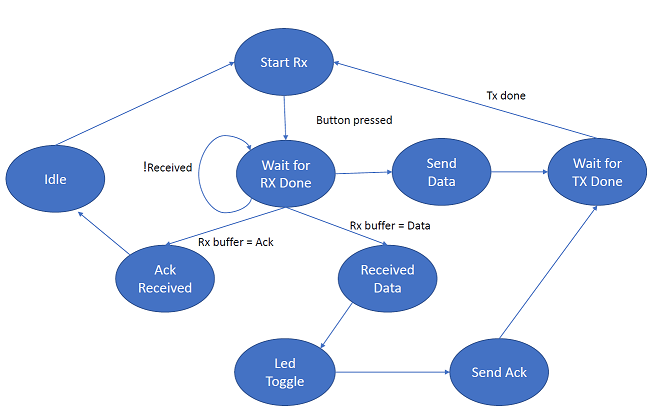
\includegraphics[scale=0.8]{img/p2p_fsm.PNG}
  \end{center}
  \fonte{HT Micron\cite{HTSXMO32L} }
  \label{fig:p2p}
\end{figure}

Este algorítimo basicamente mantém o seu rádio receptor sempre ativo e é capaz de ligar o transmissor a qualquer momento a partir de um evento de botão. Dentre as alterações necessárias para operação de acordo com este trabalho, destaca-se a alteração da funcionalidade do botão para simular eventos do sistema de \textit{Wake-up Receiver}. Desta forma, pode-se medir tanto a quantidade de energia dos seguintes estados de operação:
\begin{itemize}
    \item Modo profundo de economia de energia
    \item Consumo do receptor ligado por segundo
    \item Consumo durante a transmissão de dados
    \item Consumo para escrita na memória
    \item Consumo para conversa com o RTC
\end{itemize}

Sequencialmente pode-se definir um protocolo de comunicação para estabelecer os dois comandos descritos no fluxograma de operação para inicializar uma nova medição e para coletar os dados armazenados durante o processo de transporte.

Alternativamente, pode-se reduzir o a potência do rádio para obter melhores resultados em termos de economia de energia, já que o uso da rede Sigfox não se faz necessária para envio de dados e sim o uso de um dispositivo projetado especificamente para coleta e inicio de operação.

%%%%%%%%%%%%%%%%%%%%%%%%%%%%%%%%%%%%%%%%%%%%%%%%%%%%%%%%%%%%%%%%%%%%%%